\chapter{Implementation}

From the background research, it is clear there are a number of existing projects which to some extent achieve a component of the desired solution for this project. Scratch and Blockly enable a non-technical user to drag and drop interlocking blocks to make programs, however these programs are limited in usefulness, and are not compatible with objects in an object-oriented language.\par
Many JSON parsers exist for different languages, however most do not allow duplicate keys in objects, so can not be used. The GSON library enables object serialisation and deserialisation, but the deserialisation does not use object constructors. This means it is limited for use for data objects only, and therefore can not be used in the solution. Also, GSON supports deserialization only of JSON objects, while the solution supports JSON values and JSON arrays as well. A combination of these ideas is used to realise a solution.

\section{Parser}

Once the non-technical user has created their program, it first must be parsed and stored in data structures in Java. The grammar for JSON was obtained from the official JSON website \cite{json}. This is shown in figure \ref{fig:json_grammar}.
\begin{figure}
    \centering
    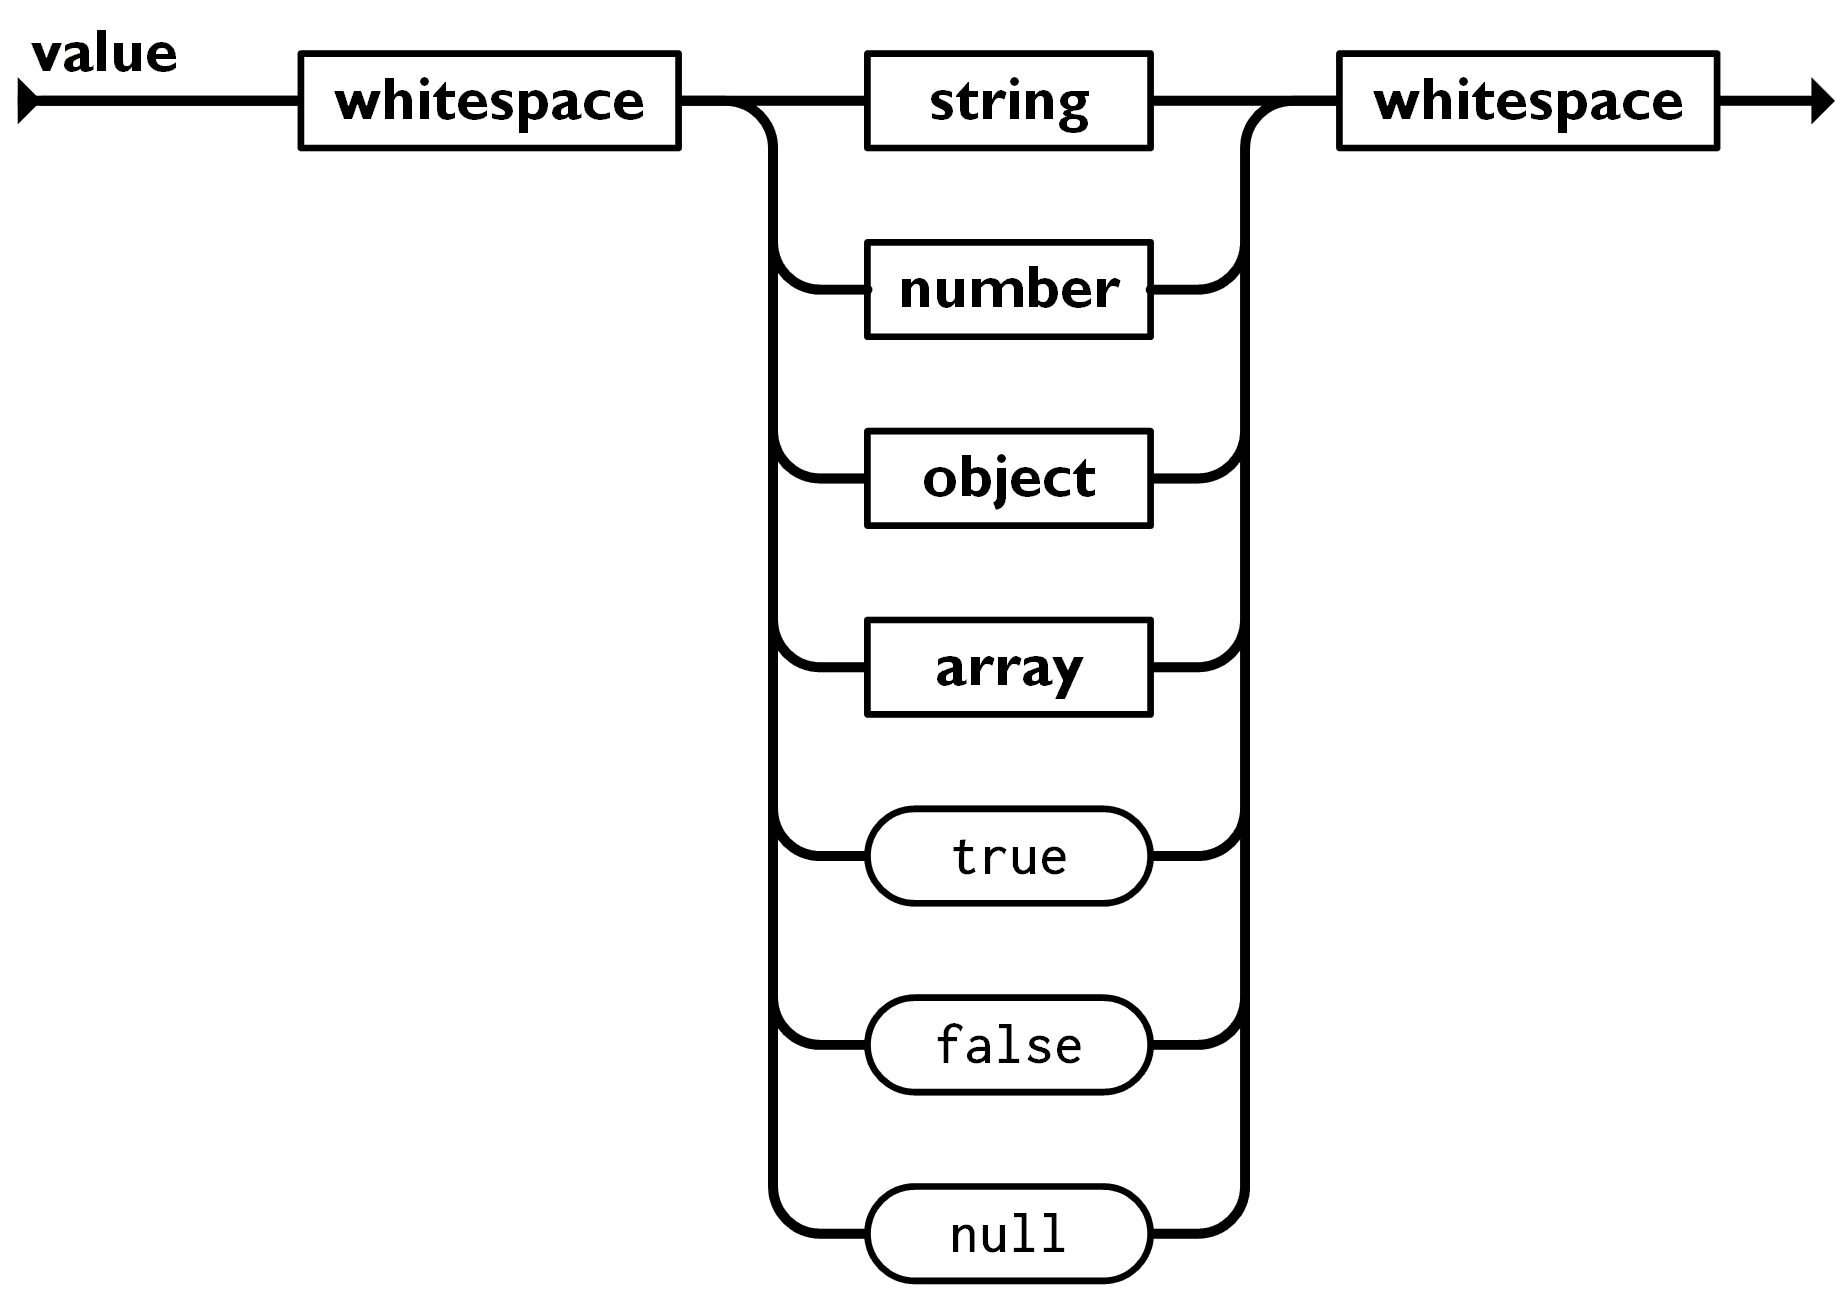
\includegraphics[width=1.0\textwidth]{Figures/json-grammar.png}
    \caption{JSON Grammar}
    \label{fig:json_grammar}
\end{figure}
\subsection{Grammar}
For the reasons previously discussed, JavaCC was chosen to create the parser. JavaCC accepts a grammar in EBNF form. It has its own file type, with the extension .jj. This file is then used to generate Java source files containing the compiler. First, tokens for quotes, commas, colons, brackets and digits were created. An integer was defined as an optional minus sign, followed by at least one digit:
\begin{verbatim}
< INTEGER : ("-")? (< DIGIT >)+ >
\end{verbatim}
A decimal is defined as an optional minus, followed by any number of digits, followed by a decimal place, followed by at least one digit:
\begin{verbatim}
< DECIMAL : ("-")? (< DIGIT >)* “.” (< DIGIT >)+ >}
\end{verbatim}
A string was defined as a quote, followed by any number of characters that are not quotes, followed by a quote:
\begin{verbatim}
< STRING : < QUOTE > (~[ "\"" ])* < QUOTE > >
\end{verbatim}
The parser was set to skip white spaces, new lines characters, and tabs. The first step was to parse JSON values, which can be a boolean, number, or string. Null values were omitted as non-technical users would not be aware of the concept of null. Boolean values were easily parsed using the true and false tokens. Integers and decimals were parsed using the BigInteger and \texttt{BigDecimal} objects respectively. These objects are built into Java, and allow very large numbers, that are above 64 bits, to be stored \cite{big_integer_big_decimal}.\par
It was worth considering whether it was logical to create new data objects specifically for the parser (some parsers have a JsonElement, JsonArray, etc objects). This can make the parser cleaner and more easier for a developer to use as an API. However since this parser is used only internally in the solution to initialise Java objects, it is not required. It would also add unnecessary overhead to the project, as the Java standard library supports all data structures required. Strings were parsed using the string token, with the opening and closing quotes removed.
\subsection{List Parsing}
The next logical thing to parse was a JSON list or array. JSON lists start with an opening square bracket \texttt{[}, have a sequence of JSON elements (can be a JSON value, another JSON list, or JSON object), and end with a closing square bracket \texttt{]}. Empty lists are allowed. The ArrayList data structure in Java was used to store the list. It is the most commonly used list data structure in Java, and allows the underlying array to be dynamically resized as elements are added \cite{array_list}. This is shown in figure \ref{fig:array_parsing}.
\begin{figure}
\centering
\caption{Array Parsing}
\label{fig:array_parsing}
\begin{verbatim}
List<Object> array() :
{
  List<Object> array = new ArrayList<Object>();
  Object element;
}
{
  < BRACKET_OPEN >
  (
    element = element()
    {
      array.add(element);
    }
    (
      < COMMA > 
      element = element()
      {
        array.add(element);
      }
    )*
  )?
  < BRACKET_CLOSE >
  {
    return array;
  }
}
\end{verbatim}
\end{figure}

\subsection{Object Parsing}
JSON objects are similar to JSON lists, however each element has both a key and corresponding value. As previously discussed, the parser would need to allow duplicate keys in objects. Usually JSON parser implementations use a map or dictionary data structure to store objects, however this can obviously not be used here. Java of course has a HashMap implementation, however two identical keys will generate the same hash, so the second key-value entry would overwrite the first. One solution would be to use both the key of the entry, and its position in the parent JSON object (such as the line number) to generate the hash. Generating hashes in this way allows the map to store multiple entries with keys of the same name, as the hash is generated off both the key and its position in the file.\par
The Google Guava library implements a HashBasedTable \cite{hash_based_table}, which allows a composite key to be generated based off of two keys. However, this data structure does not preserve insertion order, meaning object representations would lose their ordering with respect to each other. Therefore HashBasedTable can not be used in the solution. Also, this would mean any time a lookup was performed on a JSON object to get the corresponding value of a given key, both the key and its position in the file would be needed, which is inconvenient.\par
A more logical data structure for storing a JSON object is a list of key-value entries. The downside of this is that the lookup for a value of a given key is slower, O(n) in the worst case, instead of O(1) if a hash map was used. However this inefficiency is fairly insignificant, as the data structure will only be used internally. Firstly, it is used to sequentially iterate through the sequence of object representations in the file. And secondly, if the value of an entry is a JSON object, that JSON object will be used to find and initialise the correct constructor of the Java class.\par
When this is the case, the number of entries in the object will be the number of parameters in the Java class constructor, which will likely not be a large number. In other words, for what the parser is used for, there is no case where it will be required to get the value of a given key within a large JSON object, meaning there is not an issue in using this data structure.\par
The list of entries data structure for an object can be thought of as entries with pointers to the succeeding entry. A linked list stores elements by having each element have a pointer pointing to the next element. This makes it a logical choice to use as a data structure for a JSON object. It also allows the ability to distinguish between whether a list is in fact a JSON list, or JSON object, by checking if it is an instance of ArrayList or LinkedList respectively. JSON objects were parsed similarly to JSON lists, but obviously using key-value entries rather than single elements. This is shown in figure  \ref{fig:object_parsing}.
\begin{figure}
\centering
\caption{Object Parsing}
\label{fig:object_parsing}
\begin{verbatim}
List<Entry<String, Object>> object() :
{
  List<Entry<String, Object>> object =
  new LinkedList<Entry<String, Object>>();
  String key;
  Object value;
}
{
  < BRACE_OPEN >
  (
    key = string() < COLON > value = element()
    {
      object.add(Entry.of(key, value));
    }
    (
      < COMMA > 
      key = string() < COLON > value = element()
      {
        object.add(Entry.of(key, value));
      }
    )*
  )?
  < BRACE_CLOSE >
  {
    return object;
  }
}
\end{verbatim}
\end{figure}

\subsection{Parser Compilation}
At this stage the parser was almost complete. The root of any JSON parse tree is a JSON list or JSON object. The parser was set to start with initially parsing either a JSON list or JSON object, and then recursively parse the remaining structure of the JSON. The Java files for the parser were compiled from the JavaCC file and added to the project.

\section{Object Initialisation}

At this stage, the contents of a JSON file containing the representation of a program can be parsed and stored in data structures in Java. The next stage was to take this data and use it to actually initialise classes, creating object instances. The first step is to determine what classes this can be done for. As previously discussed, these types of classes are referred to as ‘blocks’, to help the understanding of non-technical users. The solution includes a standard library of blocks that can be used universally, such as the \texttt{SetAttribute} block, which sets some attribute of the program, such as its name or author. Another example is the \texttt{Wait} block, which makes the program wait a specified amount of time before the client is progressed to the next block. While these blocks serve their purpose, the project must have an API to hook into existing software libraries to maximise its usefulness. Hence, the API must allow the ability to add more blocks.\par
\subsection{Adding Custom Block Classes}
To allow custom block classes to be added, the project is compiled to a jar. Then, other projects are able to use the jar as a dependency, meaning they can add their own block classes. In a Java project, it is not possible to gain a list of all classes in the project \cite{java_classes_in_package}, even with reflection. If this was the case, it would be possible to simply make every object able to be initialised. The problem with this, even if it was possible, would be that there are many circumstances where you would not want all classes to be able to be initialised. For example, if the project has two classes of the same name but in different packages, it would be impossible to determine which class should be initialised, since the JSON representation specifies only the class name, not the package of the class. Obviously it is possible to register individual classes to be block classes, and the solution does support this. However, this is tedious if there is a large number of classes to be registered. The ability to register all classes in a package to become block classes would solve this. Java classes are organised into packages, corresponding to the folder structure of the project.
\subsection{Retrieving Classes in a Package}
It is not possible to get all classes contained in a package in Java, even with reflection. However since packages correspond to the folder structure of the source code, or of the jar if it's compiled, a workaround is possible. After some research and experimentation, two solutions were devised, depending on whether the code is compiled in a jar, or run directly from an integrated development environment. The first step is to check if the code is running in a jar, by checking if a jar file exists:
\begin{verbatim}
new File(ClassUtils.class.getProtectionDomain().getCodeSource()
.getLocation().toURI())
\end{verbatim}
If this returns true, the internal structure of the jar can be traversed using the \\\texttt{java.util.jar.JarFile} class, and the names of all .class files in a given package can be extracted as shown in figure \ref{fig:classes_in_package_jar}.
\begin{figure}
\centering
\caption{Retrieval of classes in a package in a jar}
\label{fig:classes_in_package_jar}
\begin{verbatim}
Set<Class<?>> getClassesFromJar(File jarFile, String packageName) {
  Set<Class<?>> classes = new HashSet<Class<?>>();
  try {
    JarFile file = new JarFile(jarFile);
    for (Enumeration<JarEntry> entry = file.entries(); 
entry.hasMoreElements();) {
      JarEntry jarEntry = entry.nextElement();
      String name = jarEntry.getName().replace("/", ".");
      if (name.startsWith(packageName) && name.endsWith(".class")) {
        classes.add(Class.forName(name.substring(0, name.length() - ".class".length())));
      }
    }
    file.close();
    } catch (Exception exception) {
      exception.printStackTrace();
    }
    return classes;
}
\end{verbatim}
\end{figure}
The second solution is required if the code is not compiled in a jar. This solution uses the reflections library, which extends the capabilities of standard Java reflection. It allows for runtime metadata analysis, scanning of the classpath, indexing metadata, and allows the ability to query on runtime \cite{reflections}.
At this point, the project needed to depend on this library. Apache Maven is a software project management and comprehension tool. Based on the concept of a project object model (POM), Maven can manage a project's build, reporting and documentation from a central piece of information \cite{maven}. The project was converted from a standard Java project to a Maven Java project. By adding the following XML to the project’s pom.xml file, the reflections library was automatically compiled into the project jar whenever it was built:
\begin{verbatim}
<dependency>
  <groupId>org.reflections</groupId>
  <artifactId>reflections</artifactId>
  <version>0.9.12</version>
  <scope>compile</scope>
</dependency>
\end{verbatim}
The classes in a package can be retrieved using the reflections library and \texttt{ClassLoader} as shown in figure  \ref{fig:classes_in_package_outside_jar}.
\begin{figure}
\centering
\caption{Retrieval of classes in a package outside a jar}
\label{fig:classes_in_package_outside_jar}
\begin{verbatim}
Set<Class<?>> getClassesFromClassLoader(String packageName) {
    List<ClassLoader> classLoadersList = new LinkedList<ClassLoader>();
    classLoadersList.add(ClasspathHelper.contextClassLoader());
    classLoadersList.add(ClasspathHelper.staticClassLoader());

    ConfigurationBuilder config = new ConfigurationBuilder();
    // don't exclude Object.class
    config.setScanners(new SubTypesScanner(false), new ResourcesScanner());
    // filter package
    config.filterInputsBy(new FilterBuilder()
    .include(FilterBuilder.prefix(packageName)));
    config.setUrls(ClasspathHelper.forJavaClassPath());

    return new Reflections(config).getSubTypesOf(Object.class);
}
\end{verbatim}
\end{figure}
Initially, the line
\begin{verbatim}
config.setUrls(ClasspathHelper.forJavaClassPath())
\end{verbatim}
was
\begin{verbatim}
config.setUrls(ClasspathHelper.forClassLoader(classLoadersList
.toArray(new ClassLoader[0])));
\end{verbatim}
However, the latter did not work when testing on a macOS due to differences in the Java Virtual Machine and class loader. After brief research, the corrected version was found.\par
The two solutions outlined above were combined, so that the classes in a package could be retrieved in any circumstance. This allowed the API to have a method to register all classes in a given package as block classes.
\subsection{Program Loading}
Now that the block classes could be determined, the next stage was to initialise these classes using the JSON representation. Initially, the API required setting a folder containing all JSON files to be loaded, and then a \texttt{load()} method called. However, it made more intuitive sense to have a single \texttt{load} method which takes a folder as an argument. All files contained in the folder are retrieved recursively using the method shown in figure \ref{fig:files_in_folder}.
\begin{figure}
\centering
\caption{Obtaining files in a folder recursively}
\label{fig:files_in_folder}
\begin{verbatim}
Set<File> getFiles(File folder) {
  Set<File> files = new HashSet<>();

  if (!folder.isDirectory()) {
    return files;
  }

  for (File file : folder.listFiles()) {
    if (file.isDirectory()) {
      files.addAll(getFiles(file));
    } else {
      files.add(file);
    }
  }

  return files;
}
\end{verbatim}
\end{figure}
\par
The files with a \texttt{.json} or \texttt{.blox} extension are loaded in alphabetical order, which allows non-technical users to ensure a given program gets loaded after any programs it depends on. If the file does not have valid JSON (the parsing fails) or it is not a JSON object, an \texttt{IllegalStateException} is thrown. Each key-value entry is parsed and converted into an object instance. The key is used to determine the block class used for initialisation. In order to allow maximum flexibility, the key is converted to lowercase (as block classes are registered using a lowercase key), and spaces are removed. In other words, both:
\begin{verbatim}
{
“MyObject1”:argument
}
\end{verbatim}
and...
\begin{verbatim}
{ 
“my object 1”:argument
}
\end{verbatim}
work and initialise the same object. This allows for representations to be closer to natural language. For example:
\begin{verbatim}
{
“Show home screen”:[]
}
\end{verbatim}
Will result in the initialisation of a block class named \texttt{ShowHomeScreen}.\par
Each key-value entry is then used to initialise a new object using the representations previously discussed. If a class of the given name is not found, an exception is thrown. First, a list of parameters is created. If the value of the entry is a single JSON primitive value (boolean, number or string) and not a collection (JSON list or JSON object), then that single value is extracted and added to the parameter list.\par
Values are extracted by checking if its class type is a boolean, number or string. Primitive wrapper classes  are converted into the equivalent primitive class when the type of a constructor parameter is primitive. For example, if a constructor has a parameter of type \texttt{int}, and the extracted value is of type \texttt{Integer}, the value will be converted from being an \texttt{Integer} type to an \texttt{int} type. Additionally, if a constructor parameter type is a decimal type, such as float or double, and the supplied parameter is an integer, the parameter is converted to a decimal type. This is shown in figure  \ref{fig:number_cast}.
\begin{figure}
\centering
\caption{Number Casting}
\label{fig:number_cast}
\begin{verbatim}
Object castNumber(Class<?> requiredParameter, Object parameter) {
    Class<?> suppliedParameter = parameter.getClass();

    // casts numbers to the specified type
    if (requiredParameter == double.class) {
        if (suppliedParameter == int.class || 
suppliedParameter == Integer.class) {
            return (double) ((int) parameter);
        }
    } else if (requiredParameter == float.class) {
        if (suppliedParameter == int.class || 
suppliedParameter == Integer.class) {
            return (float) ((int) parameter);
        } else if (suppliedParameter == double.class || 
suppliedParameter == Double.class) {
            return (float) ((double) parameter);
        }
    }

    return parameter;
}
\end{verbatim}
\end{figure}

These kinds of operations are performed by the Java compiler itself, which gives the language more flexibility. However, since it is obviously not possible to access elements of the Java compiler from Java runtime, these operations must be replicated at a higher level.\par

Once the parameters have been collected, a search is performed to find a constructor of the class whose parameter types match the closest to the supplied parameter types. This is done using the  algorithm shown in figure \ref{fig:best_constructor}.
\begin{figure}
\centering
\caption{Best constructor retrieval}
\label{fig:best_constructor}
\begin{verbatim}
Constructor<?> getConstructor(Class<?> clazz, List<Object> parameters, 
boolean lenient) {
    search: for (Constructor<?> c : clazz.getConstructors()) {
        int numParameters = c.getParameterTypes().length;

        // don't require array parameter
        if (numParameters > 0 && 
c.getParameterTypes()[c.getParameterTypes().length - 1].isArray()) {
            numParameters--;
        }

        // continue if not enough parameters
        if (parameters.size() < numParameters) {
            continue;
        }

        // check parameter types equal
        for (int i = 0; i < Math.min(c.getParameterTypes().length, 
parameters.size()); i++) {
            Class<?> requiredParameter = c.getParameterTypes()[i];

            // fix parameter if it is an array
            boolean array = requiredParameter.isArray() && 
            i == c.getParameterTypes().length - 1;
            requiredParameter = array ? requiredParameter.getComponentType() :
            requiredParameter;

            // if array, check all remaining parameters equal the array type
            for (int j = i; j < (array ? parameters.size() : i + 1); j++) {
                Class<?> suppliedParameter =
                castClass(parameters.get(j).getClass());

                if (!suppliedParameter.equals(requiredParameter)) {

                    // if lenient, try number casting to make parameter types match
                    if (lenient) {
                        Object number = castNumber(requiredParameter, 
                        parameters.get(j));
                        suppliedParameter = castClass(number.getClass());

                        if (suppliedParameter.equals(requiredParameter)) {
                            // update parameters with casted number
                            parameters.set(j, number);
                            continue;
                        }
                    }

                    continue search;
                }
            }
        }

        return c;
    }
    return null;
}
\end{verbatim}
\end{figure}
\subsection{Representation Flexibility}
The algorithm allows for constructors which have an array type for their final parameter to be initialised. In other words, this allows constructors such as:
\begin{verbatim}
public DisplayMessage(String... messages) {
...
}
\end{verbatim}
to be initialised using any of the following representations:
\begin{verbatim}
“DisplayMessage”: []
\end{verbatim}
(with no arguments)
\\
\begin{verbatim}
“DisplayMessage”: “Message”
\end{verbatim}
(with a single argument)
\\
\begin{verbatim}
“DisplayMessage”: [ “Line 1”, “Line 2” ]
\end{verbatim}
(with multiple arguments)
\\\\
One of the core philosophies decided whilst developing the project was to allow maximum flexibility, and enforce minimal verbosity on the non-technical user. Giving non-technical users this leeway maximises the amount of time they spend on creating programs, as they are not wasting time fixing formatting problems. It also allows the representation to be slightly closer to natural language, which as previously mentioned, is one of the goals of the project.\par

The lenient parameter of the algorithm is optional, but if specified, will make a greater effort to find the correct parameter type. This is achieved by attempting to cast number types to match the types of the constructor parameters. The solution runs the algorithm once with lenient set to false, to try and find the correct constructor with maximum precision. If the algorithm is unsuccessful, it is run again with lenient set to true. If it is still unsuccessful in finding a constructor, the provided representation does not match the class, and an \texttt{IllegalArgumentException} is thrown.\par

If the constructor found has an array type as its last parameter as mentioned, the arguments  are converted accordingly, with the last n arguments converted to a single array argument. This is achieved using the algorithm shown in figure  \ref{fig:arguments_to_array}.
\begin{figure}
\centering
\caption{Multiple argument to single array conversion}
\label{fig:arguments_to_array}
\begin{verbatim}
// if last argument of constructor is an array, convert
Class<?>[] paramTypes = constructor.getParameterTypes();
if (paramTypes.length > 0 && paramTypes[paramTypes.length - 1].isArray()) {
    List<Object> typeArray = new ArrayList<>();

    // remove parameters that form an array
    if (parameters.size() >= paramTypes.length) {
        for (int i = paramTypes.length - 1; i < parameters.size(); i++) {
            typeArray.add(parameters.get(i));
        }
        for (int i = parameters.size() - 1; i >= paramTypes.length - 1; i--) {
            parameters.remove(i);
        }
    }

    // create array and add to the parameters
    Class<?> arrayTest = paramTypes[paramTypes.length - 1];

    if (arrayTest.getComponentType().isPrimitive()) {
        parameters.add(createPrimitiveArray(typeArray, arrayTest));
    } else {
        parameters.add(typeArray.toArray((Object[]) 
Array.newInstance(arrayTest.getComponentType(), typeArray.size())));
    }
}
\end{verbatim}
\end{figure}

This is represented visually in figure  \ref{fig:arguments_to_array_visual}.

\begin{figure}
\centering
\caption{Multiple argument to single array conversion}
\label{fig:arguments_to_array_visual}
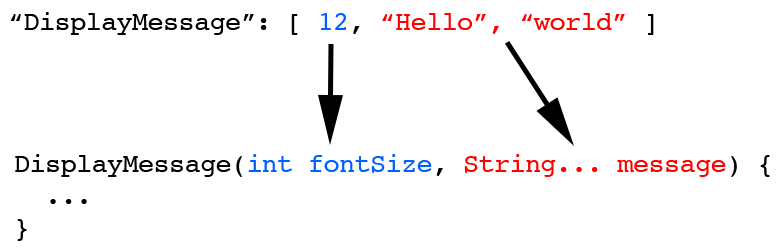
\includegraphics[width=0.7\textwidth]{Figures/array.png}
\end{figure}

Finally, the constructor is initialised and added to a list of the projects that have been initialised from the file.\par

As previously discussed, a JSON object is stored using a Java \texttt{LinkedList}, a list of key-value entries linking to each other. This means the representation can be checked to see if it is a JSON object by simply checking if it is an instance of \texttt{LinkedList}. In this case, the correct constructor for the class can be determined more accurately. This is because it is possible to search for a constructor based on the names of its parameters as well as the types of its parameters. The parameter names are checked first, as they are string types, and strings can be compared with less ambiguity and complexity than types. This is done using the algorithm displayed in figure  \ref{fig:json_object_to_java_object}.
\begin{figure}
\centering
\caption{Instantiation from JSON object representation}
\label{fig:json_object_to_java_object}
\begin{verbatim}
Map<String, Object> object = new HashMap<>();
for (Entry<String, Object> keyValue : (List<Entry<String, Object>>) value) {
    // add parameter name-value pairs to map
    object.putIfAbsent(keyValue.getKey().toLowerCase(), 
extractParameter(keyValue.getValue(), true));
}

// search for suitable constructor
constructors: for (Map.Entry<Constructor<?>, List<String>> entry : 
blockConstructors.get(blockClass).entrySet()) {
    // check if parameter names equal
    if (!object.keySet().equals(entry.getValue().stream().collect(Collectors.toSet()))) {
        continue;
    }

    // clear parameters from previous attempts
    parameters.clear();

    // check if parameter types equal
    Class<?>[] paramTypes = entry.getKey().getParameterTypes();
    List<String> paramNames = entry.getValue();

    for (int i = 0; i < paramTypes.length; i++) {
        String paramName = paramNames.get(i);
        Object suppliedParam = object.get(paramName);
        Class<?> suppliedClass = castClass(suppliedParam.getClass());

        // nested block
        if (suppliedParam instanceof LinkedList) {
            suppliedParam = getBlock(paramTypes[i], suppliedParam);
        } else {
            // cast number to match type
            suppliedParam = castNumber(paramTypes[i], suppliedParam);
        }

        // check parameter types equal
        if (!suppliedClass.equals(paramTypes[i])) {
            continue constructors;
        }

        // add parameter
        parameters.add(suppliedParam);
    }

    // both parameter names and type equal, save the discovered constructor and stop searching
    constructor = entry.getKey();
    break;
}
\end{verbatim}
\end{figure}
First, the list of entries is converted to a map (since this JSON object will never need to have keys with the same entries). The keys are converted to lowercase so that they can be compared to the parameters names of the constructor with case insensitivity.\par

The JSON object keys must now be compared to the parameter names of the block classes’ constructors. It is not possible to determine constructor parameter names in Java within the standard Java library, even using reflection \cite{java_constructor_parameter_names}. Again, an external library must be used. ASM is an all purpose Java bytecode manipulation and analysis framework. It can be used to modify existing classes or to dynamically generate classes, directly in binary form \cite{asm}. It enables the ability to extract constructor parameter names using the algorithm shown in figure  \ref{fig:constructor_parameter_names}.
\begin{figure}
\centering
\caption{Retrieval of constructor parameter names}
\label{fig:constructor_parameter_names}
\begin{verbatim}
List<String> getConstructorParameterNames(Constructor<?> constructor) {
    Class<?> declaringClass = constructor.getDeclaringClass();
    ClassLoader declaringClassLoader = declaringClass.getClassLoader();

    Type declaringType = Type.getType(declaringClass);
    String constructorDescriptor = Type.getConstructorDescriptor(constructor);
    String url = declaringType.getInternalName() + ".class";

    InputStream classFileInputStream = declaringClassLoader.getResourceAsStream(url);
    if (classFileInputStream == null) {
        throw new IllegalArgumentException("The constructor's class loader cannot find the bytecode that defined the constructor's class (URL: " + url + ")");
    }

    ClassNode classNode = null;
    try {
        try {
            classNode = new ClassNode();
            ClassReader classReader = new ClassReader(classFileInputStream);
            classReader.accept(classNode, 0);
        } finally {
            classFileInputStream.close();
        }
    } catch (Exception exception) {
        throw new IllegalArgumentException("Error getting constructor parameter names for " + constructor.getClass());
    }

    List<MethodNode> methods = classNode.methods;
    for (MethodNode method : methods) {
        if (method.name.equals("<init>") && method.desc.equals(constructorDescriptor)) {
            Type[] argumentTypes = Type.getArgumentTypes(method.desc);
            List<String> parameterNames = new ArrayList<String>(argumentTypes.length);

            List<LocalVariableNode> localVariables = method.localVariables;
            for (int i = 0; i < argumentTypes.length; i++) {
                // the first local variable actually represents the "this" object
                parameterNames.add(localVariables.get(i + 1).name);
            }

            return parameterNames;
        }
    }

    return null;
}
\end{verbatim}
\end{figure}
The ASM library was added to the project build in a similar fashion to the reflections library, by adding the following XML to the projects pom.xml:
\begin{verbatim}
<dependency>
    <groupId>org.ow2.asm</groupId>
    <artifactId>asm</artifactId>
    <version>7.1</version>
</dependency>
<dependency>
    <groupId>org.ow2.asm</groupId>
    <artifactId>asm-tree</artifactId>
    <version>7.1</version>
</dependency>
\end{verbatim}
The parameters names for a given class’ constructors are cached for efficiency when the class is registered as a block class. The cache is accessed when trying to find a constructor of a given block class with given parameter names. Once a constructor that has parameter names that match the keys of the JSON object is found, the types of the parameters are compared to the values of the JSON object. If the types match, the constructor is used to initialise a new instance of the class.\par

As previously discussed, JSON object representations of Java objects support nested objects. For example, the following case initialises a new instance of the MyObject1, using a constructor with a parameter of type MyObject2:
\begin{verbatim}
“MyObject1”:{
  “MyObject2”:{
  ...
  }
}
\end{verbatim}
This is implemented by recursively calling the method to initialise a block if a value inside a JSON object is another JSON object.

\section{API}

In order to maximise the usefulness of initialised classes, an API was included to increase the capabilities a developer has to design classes specifically to be used by non-technical users. Once a file is parsed and deserialised to objects, these objects are stored in a list, which is stored within a \texttt{Script} object. This object is used to run the program the file represents. The reason for naming the class \texttt{Script} rather than \texttt{Program} is to reflect the fact that the program will usually be small but flexible, and be dynamically interchangeable in runtime, much like scripts are. However since these programs are compiled, not interpreted, from a technical perspective they are still programs. The API also allows for programs to be loaded and unloaded during runtime.\par

\subsection{Block Class Interfaces}
The \texttt{Block} interface can optionally be implemented by classes registered as block classes. This allows the class to override the methods \texttt{onLoad} and \texttt{onUnload}, which are called when the program is loaded and unloaded respectively. It also gives the class access to its parent \texttt{Script} objects, which can be used to access other blocks in the program. This allows multiple blocks to be used together to provide combined functionality.\par

When programs are run, they often provide some functionality to the client. When this is the case, the idea is that the client progresses through the program one block at a time, with each block providing some behaviour for the client. Client is referred to here in abstract terms. The definition depends on what the project is being applied to. In the case of some graphical interface, the client will represent the user using the interface. In the case of a game, the client will be a player of the game. When the API is initialised, the desired class to represent the client is supplied as a generic type.\par

The \texttt{ClientBlock} interface is an extension of the \texttt{Block} interface which allows classes to implement these behaviours. The \texttt{onEnter} and \texttt{onExit} can be overridden to detect when the client enters and exits the block respectively. After the client has entered the block, it can be progressed to the next block using the \texttt{progress} method. The \texttt{onEnterScript} and \texttt{onExitScript} can be overridden to detect when a client enters and exits the program respectively. In other words, when they enter and exit any block in the program.\par

Any class can be used as a block class; they do not need to implement any interfaces from the API. However, classes that do not implement any of these interfaces will have limited functionality, and will most likely be used as data classes. Classes that implement \texttt{Block} are able to access their parent program, and classes that implement \texttt{ClientBlock} are able to provide behaviour to the client when they run the program. Hence there are three main types of block classes: data blocks that have no behaviour, program blocks that have behaviour that affects the program and other blocks within the program, and client blocks that have behaviour that affects the client.
